\documentclass{article}

\usepackage{subcaption}
\usepackage[utf8]{inputenc}
\usepackage[english]{babel}
\usepackage[backend=bibtex]{biblatex}
\usepackage{tikz}
\usepackage{xcolor}
\usepackage{multicol}
\usepackage{listings}
\usepackage{csquotes}
\usepackage[most]{tcolorbox}
\usepackage{parskip}
\usepackage{listings-rust}
\usepackage[scale=0.9]{sourcecodepro}
\usepackage{bytefield}
\usepackage{tikz}
\usepackage{adjustbox}
\usepackage{float}

\addbibresource{ref}


\usetikzlibrary{arrows, automata, positioning}

\usepackage[a4paper, total={6in, 8in}]{geometry}

\tcbset {
  base/.style={
    arc=0mm,
    bottomtitle=0.5mm,
    boxsep=1mm,
    boxrule=0mm,
    colbacktitle=black!10!white,
    coltitle=black,
    fonttitle=\bfseries,
    left=2.5mm,
    leftrule=1mm,
    right=3.5mm,
    title={#1},
    toptitle=0.75mm,
  },
    sub/.style={
        base={#1},
        colframe=black!30!white,
        top=-0.5mm,
        bottom=-0.5mm,
    },
}

\definecolor{brandblue}{rgb}{0.34, 0.7, 1}
\newtcolorbox{mainbox}[1]{
    nobeforeafter,
    colframe=brandblue,
    base={#1}
}

\newtcolorbox{subbox}[1]{
  colframe=black!30!white,
  sub={#1}
}

% warning mainbox
\newtcolorbox{warningbox}[1]{
  colframe=red,
  base={#1}
}

\usepackage{lato}
\renewcommand*\familydefault{\sfdefault}
\newcommand{\code}[1]{\texttt{#1}}
\usepackage[T1]{fontenc}
\usepackage{hyperref}
\usepackage{fancyhdr}

\pagestyle{fancy}
\fancyhf{}
\rhead{Giorgio Grigolo}
\lhead{CPS 2000: Compiler Theory and Practice}
\rfoot{Page \thepage}

\definecolor{bluekeywords}{rgb}{0.13, 0.13, 1}
\definecolor{greencomments}{rgb}{0, 0.5, 0}
\definecolor{redstrings}{rgb}{0.9, 0, 0}
\definecolor{graynumbers}{rgb}{0.5, 0.5, 0.5}


\lstset{
    commentstyle=\color{greencomments},
    keywordstyle=\color{bluekeywords},
    stringstyle=\color{redstrings},
    numberstyle=\color{graynumbers},
    % breaklines=true,
    basicstyle=\ttfamily,
    language=Rust,
    xleftmargin=.3\textwidth, xrightmargin=.3\textwidth,
    captionpos=b
}

\title{Compiling \code{ParL} to \code{PArIR} in Rust \\{\normalsize A report on the Rust
compiler for the \code{ParL} programming language.}}
\author{Giorgio Grigolo - 0418803L}
\date{}

\hypersetup{
    colorlinks=true,
    linkcolor=blue,
    filecolor=magenta,
    urlcolor=blue,
}

\begin{document}

\maketitle
\tableofcontents

\begin{abstract}
    In this report, we discuss the implementation details of a
    compiler for \code{ParL}, an expression-based strongly typed programming
    langauge. Code written in \code{ParL} is compiled to \code{PArIR}, which is
    the proprietary assembly-like language that is used to drive the
    programmable pixel art displays designed by the company \code{PArDis}. The
    \code{ParL} compiler was written in Rust, due to its strong type system and
    performance characteristics. It nwas implemented incrementally, as
    to ensure each component can be run in isolation, and is working correctly
    before moving on to the next one.
\end{abstract}

\newpage

\section{Project Structure}

\section{Lexical Analysis}

The first step in the compilation process is the lexical analysis. A recurring
theme in the implementation of this compiler is the use of \textit{abstraction}
to achieve \textit{modularity}, and simplify the implementation of the
subsequent stages. The lexical analysis is no exception to this rule.

At the highest level, the lexical analysis is implemented as a \code{Lexer}
struct, which is responsible for reading the input source code, and producing a
stream (\textit{or vector}) of tokens.

We shall start by defining the \code{Token} struct, which is a wrapper for the
different types of tokens that can be found in a \code{ParL} program. The
\code{Token} enum is defined as follows:

\begin{mainbox}{}
    \begin{lstlisting}
pub struct Token {
    pub kind: TokenKind,
    pub span: TextSpan,
}
    \end{lstlisting}
\end{mainbox}

The \code{TextSpan} struct is mainly used to store the lexeme of the token, and
its poosition in the source code, which is useful for error reporting. The
\code{TokenKind} is just an enum, which represents the different types of tokens, such as \code{Identifier},
\code{IntegerLiteral}, \code{If} and many more.


The actual \code{Lexer} struct is defined as follows:

\begin{mainbox}{}
    \begin{lstlisting}[caption={The \code{Lexer} struct.}]
pub struct Lexer<B: Stream> {
    buffer: B,
    dfsa: Dfsa,
}
    \end{lstlisting}
\end{mainbox}

The \code{Lexer} struct is generic over the type \code{B}, which is a trait that
abstracts out the file reading logic from the lexer. This is useful for testing
purposes, as we can easily mock the file reading logic, and test the lexer in
isolation. It is also useful in case the lexer is to be improved in the future,
by using more efficient file reading logic, such as the double buffering
technique.

The functions that a struct implementing the \code{Stream} trait, which can be
seen in Listing \ref{lst:stream-trait}, are very similar to the ones proposed in
the textbook \textit{Engineering a Compiler} \cite{engineering-a-compiler}, as the
lexer algorithm also follows the pseudo-code provided in the book.

\begin{mainbox}{}
    \lstset{xleftmargin=1cm}
    \begin{lstlisting}[language=Rust,caption={The \code{Stream} trait.}]
pub trait Stream {
    fn new(input: &str, path: &Path) -> Self;
    fn rollback(&mut self);
    fn next_char(&mut self) -> char;
    fn get_line(&self) -> usize;
    fn get_col(&self) -> usize;
    fn get_input_pointer(&self) -> usize;
    fn is_eof(&self) -> bool;
    fn current_char(&self) -> char;
    fn file_path(&self) -> &str;
}
    \end{lstlisting}
    \label{lst:stream-trait}
\end{mainbox}

Of course, the \code{Lexer} that as implemented in the project, was required to
be a based on a finite state automaton, with a character table. Initially, the
DFSA was implemented manually, but as the number of tokens (and hence states)
grew it was getting harder to keep track of the transitions.

To solve this problem, together with the \code{Dfsa} struct, a
\code{DfsaBuilder} struct was implemented, which is responsible for dynamically
building the DFSA from a number of chained function calls. I will describe each
method of the \code{DfsaBuilder} struct, and how it is used, by demonstrating
the effect as it is run incrementally on an empty DFSA.

\newpage

\subsection{DFSA Builder}

The \code{DfsaBuilder} struct is defined as follows:

\begin{mainbox}{}
    \lstset{xleftmargin=0cm}
    \begin{lstlisting}
pub struct DfsaBuilder {
    pub max_state: i32,
    pub accepted_states: Vec<i32>,
    pub character_table: HashMap<char, Category>,
    pub transition_table: HashMap<(i32, Category), i32>,
    pub state_to_token: HashMap<i32, TokenKind>,
}
    \end{lstlisting}
\end{mainbox}

Clearly, we can see that states are represented by \code{i32} integers, and
transitions are represented by a tuple of the current state and the category of
the character that is being read. The category of a character is defined by the
\code{Category} enum, containing variants such as \code{Digit}, \code{Letter},
\code{Whitespace}, and many more.


The first function is $$\code{add\_category(\&mut self, range: Vec<char>,
        category: Category)}$$  This method is used to add multiple characters to the
same category.  For example, we can add all the digits to the \code{Digit}
category, by calling \code{add\_category('0'..='9', Category::Digit)}. Note that
in the actual implementation, the \code{range} parameter is actually a more
complex type, but for simplicity's sake it can be thought of a vector. It
actually accepts anything that can be casted to an iterator, as to allow for
more convenient usage. This is done using Rust's built in ranges like
\code{'0'..='9'}. As it does not have any effect on the DFSA, but only modifies
the character table, a DFSA will not be shown.

Then, we have $$\code{add\_transition(\&mut self, state: i32, category:
        Category, next\_state: i32)}$$ This method is used to add a transition from one
state to another, given a category. For example, we can add a transition from
state 0 to state 1, when reading a digit, by calling \code{add\_transition(0,
    Category::Digit, 1)}. Note that it doesn't automatically make the state 1 an
accepted state, as it is only responsible for adding transitions.


\begin{figure}[H]
    \begin{subfigure}[t]{0.5\textwidth}
        \centering
        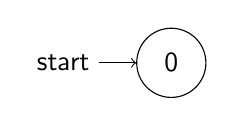
\begin{tikzpicture}
            \node[state, initial] (0) {0};
        \end{tikzpicture}
        \caption{The DFSA before adding calling \code{add\_transition}}
    \end{subfigure}
    \begin{subfigure}[t]{0.5\textwidth}
        \centering
        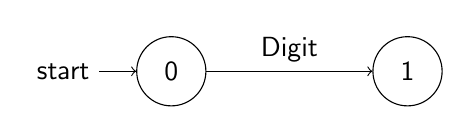
\begin{tikzpicture}
            \node[state, initial] (0) {0};
            \node[state, right of=0, xshift=2cm] (1) {1};
            \draw (0) edge[above, ->] node{Digit} (1);
        \end{tikzpicture}

        \caption{The DFSA after adding calling \code{add\_transition}}
    \end{subfigure}
\end{figure}

The next function is $$\code{auto\_add\_transition(\&mut self, state: i32,
        category: Category}$$
$$\code{to: Option<i32>, token\_kind: TokenKind) -> i32}$$

This method is used used to add a transition from \code{(state, category)} to
the state \code{to}. Since \code{to} is an \code{Option}, it can be \code{None},
in which case the destination state is automatically set to the next state. This
is useful for adding transitions to the same state, as well as constructing
slightly more complicated sequences of transitions, say for tokenizing a float.
The \code{token\_kind} parameter is used to set the token kind of the state, if
it is an accepted state. Similarly to the \code{to} parameter, it can be
\code{None}, in which case the destination state is not an accepted state.  We
also note that this function returns an integer, which is the state that was just added, for
further use in subsequent calls.

If we run \code{auto\_add\_transition(2, Category::Digit, None, Category::Float)}, the resultant DFSA will be as follows:

\begin{figure}[H]
    \begin{subfigure}[t]{0.5\textwidth}
        \centering
        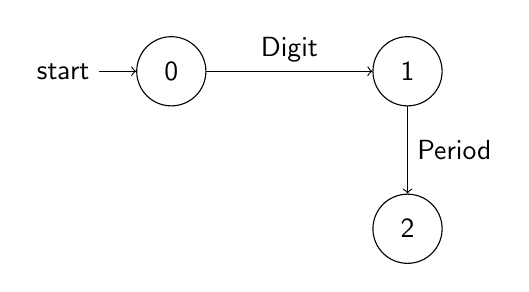
\begin{tikzpicture}
            \node[state, initial] (0) {0};
            \node[state, right of=0, xshift=2cm] (1) {1};
            \node[state, below of=1, yshift=-1cm] (2) {2};

            \draw (0) edge[above, ->] node{Digit} (1)
            (1) edge[right, ->] node{Period} (2);
        \end{tikzpicture}
        \caption{Before running the function}
    \end{subfigure}
    \begin{subfigure}[t]{0.5\textwidth}
        \centering
        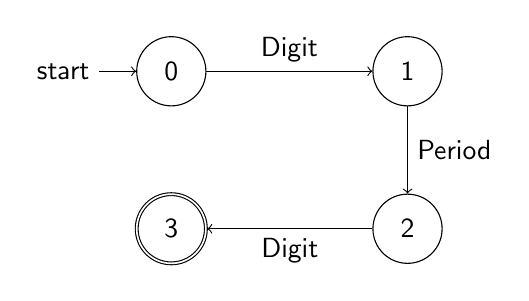
\begin{tikzpicture}
            \node[state, initial] (0) {0};
            \node[state, right of=0, xshift=2cm] (1) {1};
            \node[state, below of=1, yshift=-1cm] (2) {2};
            \node[state, accepting, below of=0, yshift=-1cm] (3) {3};

            \draw (0) edge[above, ->] node{Digit} (1)
            (1) edge[right, ->] node{Period} (2)
            (2) edge[below, ->] node{Digit} (3);
        \end{tikzpicture}
        \caption{After running the function}
    \end{subfigure}
\end{figure}

If we run \code{auto\_add\_transition(2, Category::Digit, Some(5), None)}, the
resultant DFSA will be as follows, meaning we just want to map to an auxiliary
state that doesn't correspond to any token kind, (and thus is not an accepted
state), the following is the resulting DFSA.

\begin{figure}[H]
    \begin{subfigure}[t]{0.5\textwidth}
        \centering
        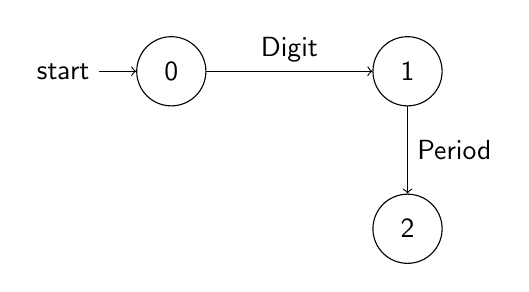
\begin{tikzpicture}
            \node[state, initial] (0) {0};
            \node[state, right of=0, xshift=2cm] (1) {1};
            \node[state, below of=1, yshift=-1cm] (2) {2};

            \draw (0) edge[above, ->] node{Digit} (1)
            (1) edge[right, ->] node{Period} (2);
        \end{tikzpicture}
    \end{subfigure}
    \begin{subfigure}[t]{0.5\textwidth}
        \centering
        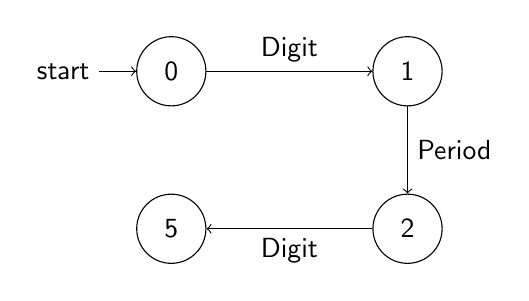
\begin{tikzpicture}
            \node[state, initial] (0) {0};
            \node[state, right of=0, xshift=2cm] (1) {1};
            \node[state, below of=1, yshift=-1cm] (2) {2};
            \node[state, below of=0, yshift=-1cm] (3) {5};

            \draw (0) edge[above, ->] node{Digit} (1)
            (1) edge[right, ->] node{Period} (2)
            (2) edge[below, ->] node{Digit} (3);

        \end{tikzpicture}
    \end{subfigure}
\end{figure}




\newpage

\printbibliography


\end{document}
